% Options for packages loaded elsewhere
\PassOptionsToPackage{unicode}{hyperref}
\PassOptionsToPackage{hyphens}{url}
%
\documentclass[
]{article}
\usepackage{amsmath,amssymb}
\usepackage{iftex}
\ifPDFTeX
  \usepackage[T1]{fontenc}
  \usepackage[utf8]{inputenc}
  \usepackage{textcomp} % provide euro and other symbols
\else % if luatex or xetex
  \usepackage{unicode-math} % this also loads fontspec
  \defaultfontfeatures{Scale=MatchLowercase}
  \defaultfontfeatures[\rmfamily]{Ligatures=TeX,Scale=1}
\fi
\usepackage{lmodern}
\ifPDFTeX\else
  % xetex/luatex font selection
\fi
% Use upquote if available, for straight quotes in verbatim environments
\IfFileExists{upquote.sty}{\usepackage{upquote}}{}
\IfFileExists{microtype.sty}{% use microtype if available
  \usepackage[]{microtype}
  \UseMicrotypeSet[protrusion]{basicmath} % disable protrusion for tt fonts
}{}
\makeatletter
\@ifundefined{KOMAClassName}{% if non-KOMA class
  \IfFileExists{parskip.sty}{%
    \usepackage{parskip}
  }{% else
    \setlength{\parindent}{0pt}
    \setlength{\parskip}{6pt plus 2pt minus 1pt}}
}{% if KOMA class
  \KOMAoptions{parskip=half}}
\makeatother
\usepackage{xcolor}
\usepackage[margin=1in]{geometry}
\usepackage{color}
\usepackage{fancyvrb}
\newcommand{\VerbBar}{|}
\newcommand{\VERB}{\Verb[commandchars=\\\{\}]}
\DefineVerbatimEnvironment{Highlighting}{Verbatim}{commandchars=\\\{\}}
% Add ',fontsize=\small' for more characters per line
\usepackage{framed}
\definecolor{shadecolor}{RGB}{248,248,248}
\newenvironment{Shaded}{\begin{snugshade}}{\end{snugshade}}
\newcommand{\AlertTok}[1]{\textcolor[rgb]{0.94,0.16,0.16}{#1}}
\newcommand{\AnnotationTok}[1]{\textcolor[rgb]{0.56,0.35,0.01}{\textbf{\textit{#1}}}}
\newcommand{\AttributeTok}[1]{\textcolor[rgb]{0.13,0.29,0.53}{#1}}
\newcommand{\BaseNTok}[1]{\textcolor[rgb]{0.00,0.00,0.81}{#1}}
\newcommand{\BuiltInTok}[1]{#1}
\newcommand{\CharTok}[1]{\textcolor[rgb]{0.31,0.60,0.02}{#1}}
\newcommand{\CommentTok}[1]{\textcolor[rgb]{0.56,0.35,0.01}{\textit{#1}}}
\newcommand{\CommentVarTok}[1]{\textcolor[rgb]{0.56,0.35,0.01}{\textbf{\textit{#1}}}}
\newcommand{\ConstantTok}[1]{\textcolor[rgb]{0.56,0.35,0.01}{#1}}
\newcommand{\ControlFlowTok}[1]{\textcolor[rgb]{0.13,0.29,0.53}{\textbf{#1}}}
\newcommand{\DataTypeTok}[1]{\textcolor[rgb]{0.13,0.29,0.53}{#1}}
\newcommand{\DecValTok}[1]{\textcolor[rgb]{0.00,0.00,0.81}{#1}}
\newcommand{\DocumentationTok}[1]{\textcolor[rgb]{0.56,0.35,0.01}{\textbf{\textit{#1}}}}
\newcommand{\ErrorTok}[1]{\textcolor[rgb]{0.64,0.00,0.00}{\textbf{#1}}}
\newcommand{\ExtensionTok}[1]{#1}
\newcommand{\FloatTok}[1]{\textcolor[rgb]{0.00,0.00,0.81}{#1}}
\newcommand{\FunctionTok}[1]{\textcolor[rgb]{0.13,0.29,0.53}{\textbf{#1}}}
\newcommand{\ImportTok}[1]{#1}
\newcommand{\InformationTok}[1]{\textcolor[rgb]{0.56,0.35,0.01}{\textbf{\textit{#1}}}}
\newcommand{\KeywordTok}[1]{\textcolor[rgb]{0.13,0.29,0.53}{\textbf{#1}}}
\newcommand{\NormalTok}[1]{#1}
\newcommand{\OperatorTok}[1]{\textcolor[rgb]{0.81,0.36,0.00}{\textbf{#1}}}
\newcommand{\OtherTok}[1]{\textcolor[rgb]{0.56,0.35,0.01}{#1}}
\newcommand{\PreprocessorTok}[1]{\textcolor[rgb]{0.56,0.35,0.01}{\textit{#1}}}
\newcommand{\RegionMarkerTok}[1]{#1}
\newcommand{\SpecialCharTok}[1]{\textcolor[rgb]{0.81,0.36,0.00}{\textbf{#1}}}
\newcommand{\SpecialStringTok}[1]{\textcolor[rgb]{0.31,0.60,0.02}{#1}}
\newcommand{\StringTok}[1]{\textcolor[rgb]{0.31,0.60,0.02}{#1}}
\newcommand{\VariableTok}[1]{\textcolor[rgb]{0.00,0.00,0.00}{#1}}
\newcommand{\VerbatimStringTok}[1]{\textcolor[rgb]{0.31,0.60,0.02}{#1}}
\newcommand{\WarningTok}[1]{\textcolor[rgb]{0.56,0.35,0.01}{\textbf{\textit{#1}}}}
\usepackage{longtable,booktabs,array}
\usepackage{calc} % for calculating minipage widths
% Correct order of tables after \paragraph or \subparagraph
\usepackage{etoolbox}
\makeatletter
\patchcmd\longtable{\par}{\if@noskipsec\mbox{}\fi\par}{}{}
\makeatother
% Allow footnotes in longtable head/foot
\IfFileExists{footnotehyper.sty}{\usepackage{footnotehyper}}{\usepackage{footnote}}
\makesavenoteenv{longtable}
\usepackage{graphicx}
\makeatletter
\def\maxwidth{\ifdim\Gin@nat@width>\linewidth\linewidth\else\Gin@nat@width\fi}
\def\maxheight{\ifdim\Gin@nat@height>\textheight\textheight\else\Gin@nat@height\fi}
\makeatother
% Scale images if necessary, so that they will not overflow the page
% margins by default, and it is still possible to overwrite the defaults
% using explicit options in \includegraphics[width, height, ...]{}
\setkeys{Gin}{width=\maxwidth,height=\maxheight,keepaspectratio}
% Set default figure placement to htbp
\makeatletter
\def\fps@figure{htbp}
\makeatother
\setlength{\emergencystretch}{3em} % prevent overfull lines
\providecommand{\tightlist}{%
  \setlength{\itemsep}{0pt}\setlength{\parskip}{0pt}}
\setcounter{secnumdepth}{5}
\usepackage[many]{tcolorbox}
\usepackage{xcolor}

\definecolor{theme}{RGB}{51, 187, 255}


\newtcolorbox{whitebox}{
  colback=white,
  colframe=theme,
  coltext=black,
  boxsep=5pt,
  arc=4pt}


\newenvironment{infobox}[1]
  {
  \begin{itemize}
  \renewcommand{\labelitemi}{
    \raisebox{-.7\height}[0pt][0pt]{
      
    }
  }
  \setlength{\fboxsep}{1em}
  \begin{whitebox}
  \item
  }
  {
  \end{whitebox}
  \end{itemize}
  }
\ifLuaTeX
  \usepackage{selnolig}  % disable illegal ligatures
\fi
\IfFileExists{bookmark.sty}{\usepackage{bookmark}}{\usepackage{hyperref}}
\IfFileExists{xurl.sty}{\usepackage{xurl}}{} % add URL line breaks if available
\urlstyle{same}
\hypersetup{
  pdftitle={Getting started with Docker},
  hidelinks,
  pdfcreator={LaTeX via pandoc}}

\title{Getting started with Docker}
\author{}
\date{\vspace{-2.5em}}

\usepackage{amsthm}
\newtheorem{theorem}{Theorem}[section]
\newtheorem{lemma}{Lemma}[section]
\newtheorem{corollary}{Corollary}[section]
\newtheorem{proposition}{Proposition}[section]
\newtheorem{conjecture}{Conjecture}[section]
\theoremstyle{definition}
\newtheorem{definition}{Definition}[section]
\theoremstyle{definition}
\newtheorem{example}{Example}[section]
\theoremstyle{definition}
\newtheorem{exercise}{Exercise}[section]
\theoremstyle{remark}
\newtheorem*{remark}{Remark}
\newtheorem*{solution}{Solution}
\let\BeginKnitrBlock\begin \let\EndKnitrBlock\end
\begin{document}
\maketitle

In this tutorial you'll learn:

\begin{itemize}
\tightlist
\item
  How to run \textbf{containers}.
\item
  How to define and build \textbf{images}.
\item
  How to create and use \textbf{volumes}.
\item
  How to define and use \textbf{networks}.
\end{itemize}

\textbf{Prerequisites:}

\begin{itemize}
\tightlist
\item
  Having installed Docker on your computer or having imported the Linux virtual machine either with VirtualBox or with Multipass.
\end{itemize}

\textbf{Related course material:}

\begin{itemize}
\item
  Slides of the first lecture. You can find them \href{https://centralesupelec.edunao.com/pluginfile.php/426017/mod_resource/content/9/cloud-cs-lecture-1.pdf}{on Edunao}.
\item
  Handbook (poly) of the first lecture. You can find it \href{https://centralesupelec.edunao.com/pluginfile.php/435165/mod_resource/content/10/chapter-1.pdf}{on Edunao}.
\end{itemize}

Using a virtual machine with Multipass? Click here for more info

\begin{infobox}{warning}

\textbf{Multipass commands}

\begin{itemize}
\item
  To start the virtual machine, type \texttt{multipass\ start\ cloudvm}.
\item
  The folder \texttt{/home/ubuntu/labs} in the virtual machine is mounted (i.e., linked) to the folder
  on YOUR computer (let's call it \texttt{LAB}) where you'll store all your lab material.
  You specified this folder when you installed the virtual machine.
\item
  If you don't remember the path to the folder linked to \texttt{/home/ubuntu/labs}, type the
  command \texttt{multipass\ info\ cloudvm}.
\item
  To open a terminal into the virtual machine, type \texttt{multipass\ shell\ cloudvm}.
\item
  When the terminal opens, the current working directory is \texttt{/home/ubuntu}.
\item
  Type \texttt{cd\ labs} to move to the folder where you'll find your lab material.
\item
  You'll use the virtual machine terminal only to type the Docker commands.
  You can use all the tools installed on your machine to create and manage the files
  in the directory \texttt{LAB} directly from your computer.
\item
  Once the lab is over, type \texttt{exit} to leave the virtual machine terminal. This will lead you back
  to the terminal of your computer.
\item
  In the terminal of your computer, type \texttt{multipass\ stop\ cloudvm} to stop the virtual machine.
  This will NOT destroy your files! It just stops the virtual machine from needlessly using the resources of your computer.
\end{itemize}

\end{infobox}

\begin{infobox}{warning}

\textbf{Terminology}

\begin{itemize}
\item
  You'll use the \textbf{terminal} to run Docker commands.
  The terminal is the \textbf{client} that communicates with
  the Docker daemon.
\item
  Docker runs \textbf{containers} on your computer.
  We'll refer to your computer as the \textbf{host},
  the containers being the \textbf{guests}.
\end{itemize}

\begin{itemize}
\tightlist
\item
  A \textbf{containerized application}
  is an application running in a container.
\end{itemize}

\end{infobox}

\section{Running containers}\label{running}

We now learn how to use the command \texttt{docker\ run} and some of
its options.
In the following exercises, we'll run containers from the image named
\emph{alpine} that is
\href{https://hub.docker.com/_/alpine}{available on the DockerHub registry}.
This image provides a lightweight distribution
(i.e., it doesn't contain many features) of Linux.

\begin{infobox}{exercisebox}

\textbf{Exercise}

\BeginKnitrBlock{exercise}
\phantomsection\label{exr:unnamed-chunk-3}{\label{exr:unnamed-chunk-3} }You want to run the container from the latest version of
the image \emph{alpine}.
Which command would you write in the terminal?
Execute it.
\EndKnitrBlock{exercise}

\end{infobox}

Solution

\begin{infobox}{exercisebox}
The goal of this exercise is to start playing with the
\texttt{docker\ run} command.
Since the question doesn't say anything about the
options, nor does it mention the command to run inside the container,
we'd type:

\texttt{docker\ run\ alpine}

\end{infobox}

\begin{infobox}{exercisebox}

\textbf{Exercise}

\BeginKnitrBlock{exercise}
\phantomsection\label{exr:unnamed-chunk-5}{\label{exr:unnamed-chunk-5} }Is the container still running?
\EndKnitrBlock{exercise}

\end{infobox}

Solution

\begin{infobox}{exercisebox}
In order to list all containers still running on the host, type the
following command:

\texttt{docker\ container\ ls}

Your container shouldn't appear in the output,
because it's not running.
In order to see all containers, including those that are not
running, type the following command:

\texttt{docker\ container\ ls\ -a}

\end{infobox}

\begin{infobox}{exercisebox}

\textbf{Exercise}

\BeginKnitrBlock{exercise}
\phantomsection\label{exr:unnamed-chunk-7}{\label{exr:unnamed-chunk-7} }By looking at the command executed within the container (\texttt{/bin/sh}),
can you tell why the container stopped without giving any output?
\EndKnitrBlock{exercise}

\end{infobox}

Solution

\begin{infobox}{exercisebox}
The command is \texttt{/bin/sh};
the container runs a Linux terminal.
But since we didn't specify what to do with that terminal
(we didn't run any Linux command, nor we tried to access the terminal),
the container stopped.

\end{infobox}

We're now going to do something useful with the image \emph{alpine}.
Make sure you read the \textbf{good practices} that you should
adopt while playing with images and containers.

\begin{infobox}{curiosity}

\textbf{Good practices}

\begin{enumerate}
\def\labelenumi{\arabic{enumi}.}
\tightlist
\item
  \textbf{Name your containers.} Although Docker assigns a default name to a new container,
  it's usually a good practice to give a container a name of your
  choice to make it easily distinguishable. You can do it by using the option
  \texttt{-\/-name}. Try the following:
\end{enumerate}

\texttt{docker\ run\ -\/-name\ my-alpine\ alpine}

As before, the container stops immediately.
If you list all your containers by typing again:

\texttt{docker\ container\ ls\ -a}

you should see a container named \emph{my-alpine}.

\begin{enumerate}
\def\labelenumi{\arabic{enumi}.}
\setcounter{enumi}{1}
\tightlist
\item
  \textbf{Remove automatically a container if you use it once.}
  Unless you want to reuse your container later, you can ask Docker to automatically remove it
  when it stops by using the option \texttt{-\/-rm}.
  This will prevent unused containers from taking up too much disk space.
\end{enumerate}

Try the following:

\texttt{docker\ run\ -\/-rm\ -\/-name\ container-to-remove\ alpine}

If you list all the containers you should see that there is no container
named \emph{container-to-remove}.

\begin{enumerate}
\def\labelenumi{\arabic{enumi}.}
\setcounter{enumi}{2}
\tightlist
\item
  \textbf{Remove unused containers.} Stopped containers that have been run without
  using the option \texttt{-\/-rm} are still stored in the host.
  If you want to remove a specific
  container (e.g., \emph{my-alpine}), use the following command:
\end{enumerate}

\texttt{docker\ container\ rm\ my-alpine}

If you want to remove all stopped containers, use the
following command:

\texttt{docker\ container\ prune}

\begin{enumerate}
\def\labelenumi{\arabic{enumi}.}
\setcounter{enumi}{3}
\tightlist
\item
  \textbf{Remove unused images.} Images can take up a lot of disk space.
  As a result, you should remember to remove those that you don't intend to use
  any longer.
  The commands to remove a specific image
  and prune unused ones are \texttt{docker\ image\ rm}
  and \texttt{docker\ image\ prune\ -a} respectively.
\end{enumerate}

\end{infobox}

\subsection{Pass a command to the containerized application}\label{pass-a-command-to-the-containerized-application}

Remember that the template of \texttt{docker\ run} is the following:

\texttt{docker\ run\ {[}options{]}\ image-name\ {[}command{]}\ {[}arg{]}}

The optional parameter \emph{command} refers to a command
that you can pass the containerized application, possibly with some arguments
(parameter \emph{arg}).

Let's see an example.
As we saw before, when we run a container from the image \emph{alpine},
a Linux terminal \texttt{/bin/sh} is launched.

\begin{infobox}{warning}

\textbf{Notice}

The Linux terminal \texttt{/bin/sh} is run within the
container.
Henceforth, we'll use the following terms:

\begin{itemize}
\tightlist
\item
  \textbf{Host terminal.} The terminal that you use to
  interact with the operating system of your computer.
\end{itemize}

\begin{itemize}
\tightlist
\item
  \textbf{Guest terminal.} The terminal that is run within
  the container.
\end{itemize}

\end{infobox}

By using the optional parameter \emph{command}, we can run
a command in the guest terminal.

\begin{infobox}{exercisebox}

\textbf{Exercise}

\BeginKnitrBlock{exercise}
\phantomsection\label{exr:command-in-guest}{\label{exr:command-in-guest} }
Run a container from the image \emph{alpine} and execute the
Linux command \texttt{ls} that lists the content of the current directory.

\begin{itemize}
\tightlist
\item
  Where are the listed files stored?
  In the host or in the container?
\end{itemize}
\EndKnitrBlock{exercise}

\end{infobox}

Solution

\begin{infobox}{exercisebox}

\texttt{docker\ run\ -\/-rm\ -\/-name\ ls-test\ alpine\ ls}

\begin{itemize}
\tightlist
\item
  The command \texttt{ls} is run in the guest terminal, therefore
  what we see in the output is a list of files stored in the
  container.
\end{itemize}

\end{infobox}

\begin{infobox}{warning}
\textbf{Notice}

In Exercise \ref{exr:command-in-guest} the command
\texttt{ls} is executed in the guest terminal, but its
output is redirected to the host terminal.

In other words, when we run the container, we
don't interact directly with the guest terminal;
we just send a command and the output is redirected
to the host terminal.

\end{infobox}

Now let's see how to execute a command in the guest terminal
that also requires an argument.

\begin{infobox}{exercisebox}

\textbf{Exercise}

\BeginKnitrBlock{exercise}
\phantomsection\label{exr:unnamed-chunk-8}{\label{exr:unnamed-chunk-8} }By using the Linux utility \texttt{ping}, check
whether the Web site \texttt{www.centralesupelec.fr} is reachable.
\EndKnitrBlock{exercise}

\end{infobox}

Solution

\begin{infobox}{exercisebox}
\texttt{docker\ run\ -\/-rm\ -\/-name\ ping-test\ alpine\ ping\ www.centralesupelec.fr}

In order to interrupt \texttt{ping}
just type the key combination that you's use to
interrupt any other command in your terminal.
(typically Ctrl-C on Windows and Cmd-C in MacOs).

\end{infobox}

Now run the following command:

\texttt{docker\ run\ \ -\/-name\ my-alpine\ -it\ alpine}

\textbf{Note:} we didn't use the option \texttt{-\/-rm} (the container will not be removed
when we stop it, we're going to use it again).
Moreover, we didn't specify any command to run in the guest terminal.

\begin{infobox}{exercisebox}

\textbf{Exercise}

\BeginKnitrBlock{exercise}
\phantomsection\label{exr:unnamed-chunk-10}{\label{exr:unnamed-chunk-10} }What do you obtain?
\EndKnitrBlock{exercise}

\end{infobox}

Solution

\begin{infobox}{exercisebox}
When we run a container from the image \emph{alpine}, the command
\texttt{/bin/sh} is executed within the container.
Since we specified the option \texttt{-it}, what we obtain is an access to the
Linux terminal running in the container.

\end{infobox}

\subsection{Starting and stopping containers.}\label{starting-and-stopping-containers.}

\texttt{docker\ run} is a shorthand for two Docker commands, namely
\texttt{docker\ create}, that creates a container from an image,
and \texttt{docker\ start}, that starts the container after its creation.

Suppose now that you want to download a Web page
by using Linux Alpine.
You can use the Linux command \texttt{wget} followed by the URL of the page
that you want to download.

\begin{infobox}{exercisebox}

\textbf{Exercise}

\BeginKnitrBlock{exercise}
\phantomsection\label{exr:wget-exo}{\label{exr:wget-exo} }By using the guest terminal
in the container \emph{my-alpine},
download
\href{https://www.centralesupelec.fr/fr/presentation}{this Web page}.

\begin{itemize}
\tightlist
\item
  Where will the Web page be saved? The host computer or the container?
\end{itemize}
\EndKnitrBlock{exercise}

\end{infobox}

Solution

\begin{infobox}{exercisebox}

Just type in \emph{my-alpine} guest terminal the following command:

\texttt{wget\ https://www.centralesupelec.fr/fr/presentation}

\begin{itemize}
\tightlist
\item
  The Web page will be saved in the current directory
  of the container. You can verify that the file is there
  by typing \texttt{ls} in the guest terminal.
\end{itemize}

\end{infobox}

Want to copy the donwloaded file from the container to your computer?

To copy the file \texttt{presentation} to your working directory, type the following command in
the host terminal:

\begin{verbatim}
  docker cp <containerId>:/presentation .
\end{verbatim}

In the previous command, replace \texttt{\textless{}containerId\textgreater{}} with the identifier of your container. You can obtain
the identifier of the container from the output of the command \texttt{docker\ container\ ls\ -a}.

\begin{infobox}{warning}

\textbf{Where are the containers and image files stored?}

If you use MacOS or Windows

The files managed by Docker are not stored directly in your computer, but
in the Linux virtual machine installed and operated by Docker Desktop (remember, Docker always need Linux to be executed).

Therefore, you need to open a terminal inside that Linux virtual machine by typing the following command:

\begin{verbatim}
docker run -it --rm --privileged --pid=host justincormack/nsenter1
\end{verbatim}

Once the terminal is opened, you can follow the instructions given below for Linux users.

If you use Docker on Linux

\begin{itemize}
\item
  All files managed by Docker are stored under folder \texttt{/var/lib/docker}.
\item
  To access that folder, you need to be root (i.e., administrator). Type the command \texttt{sudo\ su}.
\item
  If you type \texttt{ls\ /var/lib/docker} you can look at the folders stored under this directory. You'll see that there are
  folders corresponding to the different objects managed by Docker (containers, images, volumes and networks).
\item
  To locate the files of a specific container, you first need to get the \textbf{container identifier} by typing \texttt{docker\ container\ ls\ -a}.
\item
  Type the command \texttt{docker\ inspect\ \textless{}container-id\textgreater{}} (replace \texttt{\textless{}container-id\textgreater{}} with the identifier of the container that you intend to inspect).
\item
  Locate the field \texttt{UpperDir}. The value of this field is the path to the directory (let's call it \texttt{CONTAINER\_DIR}) that contains the upper layer of the container (the writable layer).
  It should be a path that ends by \texttt{/diff}.
\item
  If you type \texttt{cd\ CONTAINER\_DIR} (replace \texttt{CONTAINER\_DIR} with the value of the field \texttt{UpperDir}) you can finally see the files stored in
  your container.
\end{itemize}

\end{infobox}

In \emph{my-alpine} guest terminal type \texttt{exit}.
This closes the guest terminal and, as a result, stops the
container.

\begin{infobox}{warning}
\textbf{NOTICE}

Stopping the container will not erase any of the files
stored in the container. Removing the container will.

\end{infobox}

If you want to start the container \emph{my-alpine} again, you can
use the following command:

\texttt{docker\ container\ start\ -ai\ my-alpine}

This will open the guest terminal of the container again;
type \texttt{ls} to verify that
the Web page that you downloaded before is still there.

Homework (optional)

Suppose that you need to download all the figures of
\href{https://www.centralesupelec.fr/fr/presentation}{this Web page}.
The Linux utility \texttt{wget} comes in handy.
However, you don't have Linux and you'd like to
avoid the hassle of installing it on your computer, or in a virtual machine,
just for this task.

A great alternative is to run Linux in a Docker container.
Unfortunately, the Alpine distribution that we've been playing
with doesn't provide
an implementation of \texttt{wget} with all the options that we need.

We turn to another Linux distribution, \textbf{Ubuntu},
for which DockerHub has
\href{https://hub.docker.com/_/ubuntu/}{several images}.

\begin{infobox}{exercisebox}

\textbf{Exercise}

\BeginKnitrBlock{exercise}
\phantomsection\label{exr:unnamed-chunk-11}{\label{exr:unnamed-chunk-11} }Run a container with Ubuntu (latest) and open a guest terminal.
Call the container \emph{dl-figures}, and avoid the option
\texttt{-\/-rm}, we'll use this container later.
\EndKnitrBlock{exercise}

\end{infobox}

Solution

\begin{infobox}{exercisebox}
\texttt{docker\ run\ -\/-name\ dl-figures\ -it\ ubuntu}

\end{infobox}

From now on, we'll be interacting with the guest Ubuntu terminal.
If you type the command \texttt{wget},
you'll get an error (\texttt{bash:\ wget:\ command\ not\ found}).

\begin{infobox}{warning}
\textbf{Notice}

The image \emph{Ubuntu} doesn't include all the commands that you'd find
in a full-blown Ubuntu distribution;
the reason is to keep the size of the image small,
a necessary constraint given that
images are transferred over the Internet.

\end{infobox}

Luckily, there's a way to install \texttt{wget} in our Ubuntu distribution.
Ubuntu provides a powerful command-line package manager called
\textbf{Advanced Package Tool} (APT).
First, you need to run the following command:

\texttt{apt\ update}

which fetches the available packages from a list of sources
available in file \texttt{/etc/apt/sources.list}.

Then, you can install \texttt{wget} by running the following command:

\texttt{apt\ install\ -y\ wget}

In order to obtain all the figures from a
Web page, type the following command:

\begin{Shaded}
\begin{Highlighting}[]
\NormalTok{wget {-}nd {-}H {-}p {-}P /my{-}figures {-}A jpg,jpeg,png,gif {-}e robots=off {-}w 0.5 https://www.centralesupelec.fr/fr/presentation}
\end{Highlighting}
\end{Shaded}

You should see in the current directory a new folder
named \emph{my-figures} containing the downloaded figures;
verify it by typing \texttt{ls\ my-figures}.

Before terminating, don't forget to read your fortune cookie.
In the shell, run the following command:

\texttt{apt-get\ install\ -y\ fortune}

and then:

\texttt{/usr/games/fortune\ -s}

When you're done, you can simply type the command \texttt{exit} to quit
the guest terminal and stop the container.

\section{Creating Images}\label{creating-images}

A Docker image can be thought of as a template to create and run a container.
An image is a file that contains a \textbf{layered filesystem} with each layer being \textbf{immutable};
this means that the files that belong to a layer cannot be
modified or deleted, nor can files be added to a layer.

When a container is created from an image, it
will be composed of all the image read-only layers and, on top of
them, a writable layer (termed the \textbf{container layer}),
where all the new files created in the container will be written.
For example, the Web page that you downloaded in Exercise \ref{exr:wget-exo}
were stored in the writable layer of that container.

\subsection{Dockerfiles}\label{dockerfiles}

The most common way to create an image is to use a \textbf{Dockerfile}, a
text file that contains all the instructions necessary to
build the image.
The advantage of the Dockerfile is that it can be interpreted
by the Docker engine, which makes the creation of images an automated
and repeatable task.

Suppose that we want to create a containerized
application to download figures from a Web page.
As a template for this application, we need to build a new
image, that we'll call \emph{fig-downloader}.

The Dockerfile containing the instructions to build the image
\emph{fig-downloader} is as follows:

\begin{Shaded}
\begin{Highlighting}[]
\KeywordTok{FROM}\NormalTok{ ubuntu}
\KeywordTok{RUN} \ExtensionTok{apt{-}get}\NormalTok{ update}
\KeywordTok{RUN} \ExtensionTok{apt{-}get}\NormalTok{ install }\AttributeTok{{-}y}\NormalTok{ wget}
\KeywordTok{RUN} \FunctionTok{mkdir} \AttributeTok{{-}p}\NormalTok{ /my{-}figures}
\KeywordTok{WORKDIR}\NormalTok{ /my{-}figures}
\KeywordTok{ENTRYPOINT}\NormalTok{ [}\StringTok{"wget"}\NormalTok{, }\StringTok{"{-}nd"}\NormalTok{, }\StringTok{"{-}r"}\NormalTok{, }\StringTok{"{-}A"}\NormalTok{, }\StringTok{"jpg,jpeg,bmp,png,gif"}\NormalTok{]}
\KeywordTok{CMD}\NormalTok{ [}\StringTok{"https://www.centralesupelec.fr/fr/presentation"}\NormalTok{]}
\end{Highlighting}
\end{Shaded}

Here's the explanation:

\begin{enumerate}
\def\labelenumi{\arabic{enumi}.}
\item
  We use the image \emph{ubuntu} as the \textbf{base image}.
  This corresponds to the instruction \texttt{FROM\ ubuntu}.
\item
  We install the utility \texttt{wget} in the base image.
  This corresponds to the
  instructions \texttt{RUN\ apt-get\ update} and \texttt{RUN\ apt-get\ install\ -y\ wget}.
\item
  We create a directory \texttt{my-figures} under the root directory of the image.
  This corresponds to the instruction \texttt{RUN\ mkdir\ -p\ /my-figures}.
\item
  We set the newly created directory \emph{/my-figures} as the
  \textbf{working directory} of the image. This corresponds to the
  instruction \texttt{WORKDIR\ /my-figures}.
\item
  We specify the command to be executed when a container is run from this image.
  This corresponds to the instruction
\end{enumerate}

\texttt{ENTRYPOINT\ {[}"wget",\ "-nd",\ "-r",\ "-A",\ "jpg,jpeg,bmp,png,gif"{]}}

This instruction means: execute \texttt{wget} with the options
\texttt{-nd}, \texttt{-r}, \texttt{-A};
the last option takes a list of file
extensions (\texttt{jpg,jpeg,bmp,png,gif}) as its argument.

\begin{enumerate}
\def\labelenumi{\arabic{enumi}.}
\setcounter{enumi}{5}
\tightlist
\item
  Remember that the utility \texttt{wget} takes the URL of the Web page as
  an argument. The URL will be specified when we run the container from
  the image \emph{fig-downloader}.
  Optionally, we can specify a default argument by using the
  keyword CMD. The meaning of the instruction:
\end{enumerate}

\texttt{CMD\ {[}"https://www.centralesupelec.fr/fr/presentation"{]}}

is: if we don't give any URL when we run the container, the figures will
be downloaded from
\url{https://www.centralesupelec.fr/fr/presentation}.

\begin{infobox}{exercisebox}

\textbf{Exercise}

\BeginKnitrBlock{exercise}
\phantomsection\label{exr:unnamed-chunk-15}{\label{exr:unnamed-chunk-15} }What's the relation between the Dockerfile lines and the image layers?
\EndKnitrBlock{exercise}

\end{infobox}

Solution

\begin{infobox}{exercisebox}
Each line corresponds to a new layer.
The first line corresponds to the bottom layer;
the last line to the top layer.

\end{infobox}

\begin{infobox}{exercisebox}

\textbf{Exercise}

\BeginKnitrBlock{exercise}
\phantomsection\label{exr:dockerfile-creation}{\label{exr:dockerfile-creation} }Could you identify a problem in this Dockerfile?
Modify the Dockerfile accordingly.
\EndKnitrBlock{exercise}

\end{infobox}

Solution

\begin{infobox}{exercisebox}

When creating an image, we should keep the number of layers relatively
small; in fact, the more the layers, the bigger the image will be.
Here we create three separate layers with three RUN commands; we can
simply merge the three layers.
The resulting Dockerfile will be:

\begin{Shaded}
\begin{Highlighting}[]
\KeywordTok{FROM}\NormalTok{ ubuntu}
\KeywordTok{RUN} \ExtensionTok{apt{-}get}\NormalTok{ update }\KeywordTok{\&\&} \DataTypeTok{\textbackslash{}}
    \ExtensionTok{apt{-}get}\NormalTok{ install }\AttributeTok{{-}y}\NormalTok{ wget }\KeywordTok{\&\&} \DataTypeTok{\textbackslash{}}
    \FunctionTok{mkdir} \AttributeTok{{-}p}\NormalTok{ /my{-}figures}
\KeywordTok{WORKDIR}\NormalTok{ /my{-}figures}
\KeywordTok{ENTRYPOINT}\NormalTok{ [}\StringTok{"wget"}\NormalTok{, }\StringTok{"{-}nd"}\NormalTok{, }\StringTok{"{-}r"}\NormalTok{, }\StringTok{"{-}A"}\NormalTok{, }\StringTok{"jpg,jpeg,bmp,png,gif"}\NormalTok{]}
\KeywordTok{CMD}\NormalTok{ [}\StringTok{"https://www.centralesupelec.fr/fr/presentation"}\NormalTok{]}
\end{Highlighting}
\end{Shaded}

\end{infobox}

\subsection{Building an image}\label{building-an-image}

We're now going to build an image from a Dockerfile.

\begin{enumerate}
\def\labelenumi{\arabic{enumi}.}
\item
  Create a directory named \emph{fig-downloader} in your computer with
  a file named \emph{Dockerfile} inside.
\item
  In the \emph{Dockerfile} write the set of instructions that
  you proposed in Exercise \ref{exr:dockerfile-creation}.
\item
  In the terminal, set the working directory to \emph{fig-downloader}.
\item
  Build an image called \emph{fig-downloader} by executing the following command:
\end{enumerate}

\texttt{docker\ build\ -t\ fig-downloader\ .}

The \texttt{.} at the end of the command means that the Docker engine will
look for a file named \emph{Dockerfile} in the working directory.

\begin{infobox}{curiosity}
\textbf{Good to know}

If you give the Dockerfile a different name (say, \emph{Dockerfile-fig-downloader}),
the command to build the image will be:

\texttt{docker\ build\ -t\ fig-downloader\ -f\ Dockerfile-fig-downloader\ .}

The option \texttt{-f} is used to specify the name of the Dockerfile.

\end{infobox}

In order to verify that the new image has been created, type the following command:

\texttt{docker\ images}

\begin{infobox}{exercisebox}

\textbf{Exercise}

\BeginKnitrBlock{exercise}
\phantomsection\label{exr:dl-1-container}{\label{exr:dl-1-container} }Run the following command:

\texttt{docker\ run\ -\/-name\ dl-1\ fig-downloader}

What does it do? Where are the downloaded pictures?
\EndKnitrBlock{exercise}

\end{infobox}

Solution

\begin{infobox}{exercisebox}
We downloaded the figures
\href{https://www.centralesupelec.fr/fr/presentation}{of this page}.
The downloaded pictures are in the folder \emph{/my-figures}
of the container \emph{dl-1}.

\end{infobox}

\begin{infobox}{exercisebox}

\textbf{Exercise}

\BeginKnitrBlock{exercise}
\phantomsection\label{exr:unnamed-chunk-18}{\label{exr:unnamed-chunk-18} }Run the following command:

\begin{verbatim}
docker run --name dl-2 fig-downloader https://www.centralesupelec.fr/
\end{verbatim}

What does it do? Where are the downloaded pictures?
\EndKnitrBlock{exercise}

\end{infobox}

Solution

\begin{infobox}{exercisebox}
We downloaded the figures
\href{https://www.centralesupelec.fr}{of this page}.
We basically overwrote the URL specified by the CMD keyword with a new
one.
The downloaded pictures are in the folder \emph{/my-figures}
of the container \emph{dl-2}.

\end{infobox}

\subsection{Containerized Python application}\label{containerized-python-application}

Download \href{/courses/cloud-computing/tutorial-docker/word-frequency.zip}{this archive file}
and unzip it into your working directory.
In this archive you'll find:

\begin{itemize}
\tightlist
\item
  A Dockerfile.
\item
  A Python script \emph{main.py} that asks the user to enter the URL and the language of a Web page,
  and prints the 10 most frequent words occurring in that page.
\item
  A file \emph{requirements.txt} with the list of the Python packages
  needed to run the given script.
\end{itemize}

The content of the Dockerfile is as follows:

\begin{Shaded}
\begin{Highlighting}[]
\KeywordTok{FROM}\NormalTok{ python:3.7{-}slim}
\KeywordTok{RUN} \FunctionTok{mkdir} \AttributeTok{{-}p}\NormalTok{ /app}
\KeywordTok{WORKDIR}\NormalTok{ /app}
\KeywordTok{COPY}\NormalTok{ ./main.py ./requirements.txt /app/}
\KeywordTok{RUN} \ExtensionTok{pip}\NormalTok{ install }\AttributeTok{{-}r}\NormalTok{ requirements.txt}
\KeywordTok{ENTRYPOINT}\NormalTok{ [}\StringTok{"python"}\NormalTok{, }\StringTok{"main.py"}\NormalTok{]}
\end{Highlighting}
\end{Shaded}

\begin{infobox}{exercisebox}

\textbf{Exercise}

\BeginKnitrBlock{exercise}
\phantomsection\label{exr:unnamed-chunk-19}{\label{exr:unnamed-chunk-19} }Describe what this Dockerfile does.
\EndKnitrBlock{exercise}

\end{infobox}

Solution

\begin{infobox}{exercisebox}

\begin{itemize}
\tightlist
\item
  Takes \emph{python:3.7-slim} as the base image.
\item
  Creates a new folder \emph{app} in the image under the root directory.
\item
  Changes the working directory to \emph{/app}.
\item
  Copies the files \emph{main.py} and \emph{requirements.txt} from the local
  computer to the directory \emph{/app} in the image.
\item
  Runs the command \texttt{pip\ install} to install the Python libraries
  specified in the file \emph{requirements.txt}.
\item
  Executes the command \texttt{python\ main.py}.
\end{itemize}

\end{infobox}

\textbf{Exercise}

\BeginKnitrBlock{exercise}
\phantomsection\label{exr:unnamed-chunk-20}{\label{exr:unnamed-chunk-20} }Build an image called \emph{wordfreq} from this Dockerfile.
\EndKnitrBlock{exercise}

Solution

\begin{infobox}{exercisebox}
\texttt{docker\ build\ -t\ wordfreq\ .}

\end{infobox}

\begin{infobox}{exercisebox}

\textbf{Exercise}

\BeginKnitrBlock{exercise}
\phantomsection\label{exr:unnamed-chunk-21}{\label{exr:unnamed-chunk-21} }Without changing the Dockerfile, rebuild the same image.
What do you notice?
\EndKnitrBlock{exercise}

\end{infobox}

Solution

\begin{infobox}{exercisebox}
The build is very fast.
Since we didn't change the Dockerfile, the image
is rebuilt by using the image layers created
previously.
This is clearly indicated by the word \textbf{CACHED} written
at each layer.
Using the already stored layers is called \textbf{build cache}.

\end{infobox}

\begin{infobox}{exercisebox}

\textbf{Exercise}

\BeginKnitrBlock{exercise}
\phantomsection\label{exr:unnamed-chunk-22}{\label{exr:unnamed-chunk-22} }What happens if you modify a line in the Python script and
you rebuild the image?
\EndKnitrBlock{exercise}

\end{infobox}

Solution

\begin{infobox}{exercisebox}
Add any instruction at the end of \emph{main.py}, such as:

\begin{Shaded}
\begin{Highlighting}[]
\BuiltInTok{print}\NormalTok{(}\StringTok{"Finish!"}\NormalTok{)}
\end{Highlighting}
\end{Shaded}

then rebuild the image.
The three bottom layers are not affected by the modification, therefore
they benefit from the build cache.
Layer 4 is the first affected by the modification.
This layer, and those above, need therefore to be
rebuilt.

\end{infobox}

\begin{infobox}{exercisebox}

\textbf{Exercise}

\BeginKnitrBlock{exercise}
\phantomsection\label{exr:unnamed-chunk-23}{\label{exr:unnamed-chunk-23} }Based on the previous considerations,
can you tell what's wrong with this Dockerfile?
Modify the Dockerfile accordingly and rebuild the image.
\EndKnitrBlock{exercise}

\end{infobox}

Solution

\begin{infobox}{exercisebox}

Each time we modify \emph{main.py} and we rebuild the image,
the layer 4 and 5 are recreated, meaning that all the Python packages
are downloaded and installed.
Depending on the size and number of the packages, this might
take some while.
A better way to structure the Dockerfile is to install the
packages before copying the Python script to the image.
Here is how we should modify the Dockerfile:

\begin{Shaded}
\begin{Highlighting}[]
\KeywordTok{FROM}\NormalTok{ python:3.7{-}slim}
\KeywordTok{RUN} \FunctionTok{mkdir} \AttributeTok{{-}p}\NormalTok{ /app}
\KeywordTok{WORKDIR}\NormalTok{ /app}
\KeywordTok{COPY}\NormalTok{ ./requirements.txt /app/}
\KeywordTok{RUN} \ExtensionTok{pip}\NormalTok{ install }\AttributeTok{{-}r}\NormalTok{ requirements.txt}
\KeywordTok{COPY}\NormalTok{ ./main.py /app/}
\KeywordTok{ENTRYPOINT}\NormalTok{ [}\StringTok{"python"}\NormalTok{, }\StringTok{"main.py"}\NormalTok{]}
\end{Highlighting}
\end{Shaded}

\end{infobox}

\begin{infobox}{exercisebox}

\textbf{Exercise}

\BeginKnitrBlock{exercise}
\phantomsection\label{exr:unnamed-chunk-24}{\label{exr:unnamed-chunk-24} }Modify \emph{main.py} by adding a new line of code and rebuild the image.
What changed?
\EndKnitrBlock{exercise}

\end{infobox}

Solution

\begin{infobox}{exercisebox}
The Python packages are not reinstalled, as a result rebuilding the image\\
takes much less time than before.

\end{infobox}

Play with the application by running the following command:

\texttt{docker\ run\ -\/-rm\ -it\ \ wordfreq}

The containerized application will prompt you to insert the URL of a webpage and
the language of the page (in English).
The output will be the 20 most used words in the webpage.

\section{Data Volumes}\label{data-volumes}

In Exercise \ref{exr:dl-1-container} you've been asked to run a container named
\emph{dl-1} to download some figures from a Web page.
The figures were downloaded into the
directory \emph{/my-figures} of the container.
But we left a question unanswered.

\textbf{How do we transfer those figures from the container to the host computer?}

The solution is to use \textbf{volumes}.

\subsection{Docker volumes}\label{docker-volumes}

A volume can be seen as a virtual storage device attached to a container.
All files there are written to a volume survive the containerized application that
created them. In other words, when a container is destroyed,
all the files created by the application in the container remain in the volume.

Let's create a new Docker volume called \emph{data-volume}:

\texttt{docker\ volume\ create\ data-volume}

\begin{infobox}{curiosity}
\textbf{Good to know (advanced notion)}

\textbf{Where the data will be actually stored?}

You can inspect the new volume by typing the
following command:

\texttt{docker\ volume\ inspect\ data-volume}

A \emph{mount point} is indicated; that's the folder where the data
will be actually stored.
If your computer runs Linux, that folder will be available
on the host; if your computer runs Windows or MacOS,
you'll not find that folder on your computer.
Instead, it will be available in the virtual machine
that Docker use on MacOS and Windows.

\textbf{Do you want to see the directory? (Instructions for Windows and MacOS)}

One way to look into the hidden VM is to run
the following containerized application:

\texttt{docker\ run\ -it\ -\/-rm\ -\/-privileged\ -\/-pid=host\ justincormack/nsenter1}

This application will open a guest terminal into the VM.
You can then use the commands \texttt{cd} and \texttt{ls}
to browse to the directory indicated as the mount path
of the new volume.

\end{infobox}

\subsubsection{Sharing data}\label{sharing-data}

A Docker volume can be used to share data between containers.

\begin{infobox}{exercisebox}

\textbf{Exercise}

\BeginKnitrBlock{exercise}
\phantomsection\label{exr:unnamed-chunk-26}{\label{exr:unnamed-chunk-26} }Run a container from the image \texttt{ubuntu},
specifying the options to:

\begin{itemize}
\item
  Remove the container once its execution is over.
\item
  Interact with the guest Linux terminal in the container.
\end{itemize}

\begin{itemize}
\tightlist
\item
  Mount the volume \emph{data-volume} at the container's directory \emph{/data}.
\end{itemize}
\EndKnitrBlock{exercise}

\end{infobox}

Solution

\begin{infobox}{exercisebox}
\texttt{docker\ run\ -\/-rm\ -it\ -v\ data-volume:/data\ ubuntu}

\end{infobox}

\begin{enumerate}
\def\labelenumi{\arabic{enumi}.}
\tightlist
\item
  Type the following command in the guest Linux terminal to create a file
  \emph{test-file.txt} in the directory \emph{/data}:
\end{enumerate}

\texttt{echo\ "This\ is\ a\ new\ file"\ \textgreater{}\ /data/test-file.txt}

\begin{enumerate}
\def\labelenumi{\arabic{enumi}.}
\setcounter{enumi}{1}
\tightlist
\item
  Print to the console the content of the file with the following command:
\end{enumerate}

\texttt{cat\ /data/test-file.txt}

\begin{enumerate}
\def\labelenumi{\arabic{enumi}.}
\setcounter{enumi}{2}
\tightlist
\item
  Type \texttt{exit} to leave the guest terminal. Since we've specified the option \texttt{-\/-rm}, the container
  is \textbf{destroyed}. Now we're going to verify that \texttt{test-file.txt} is still accessible.
\end{enumerate}

\begin{infobox}{exercisebox}

\textbf{Exercise}

\BeginKnitrBlock{exercise}
\phantomsection\label{exr:unnamed-chunk-27}{\label{exr:unnamed-chunk-27} }Run a container from the image \emph{alpine:latest},
specifying the options to:

\begin{itemize}
\item
  Remove the container once its execution is over.
\item
  Interact with the guest Linux terminal in the container.
\end{itemize}

\begin{itemize}
\tightlist
\item
  Mount the volume \emph{data-volume} to the directory \emph{/my-data}
  of the container.
\end{itemize}
\EndKnitrBlock{exercise}

\end{infobox}

Solution

\begin{infobox}{exercisebox}
\texttt{docker\ container\ run\ -\/-rm\ -it\ -v\ data-volume:/my-data\ alpine}

\end{infobox}

\begin{infobox}{exercisebox}

\textbf{Exercise}

\BeginKnitrBlock{exercise}
\phantomsection\label{exr:unnamed-chunk-28}{\label{exr:unnamed-chunk-28} }Verify that you can read the file \emph{test-file.txt}.
Which folder would you look in?
\EndKnitrBlock{exercise}

\end{infobox}

Solution

\begin{infobox}{exercisebox}
We need to look in the folder \emph{/my-data} because this is where
we mounted \emph{data-volume}.

\texttt{cat\ /my-data/test-file.txt}

\end{infobox}

Type \texttt{exit} to exit the guest terminal and terminate the container.

\section{Single-Host Networking}\label{single-host-networking}

In order to let containers communicate and, therefore, co-operate,
Docker defines a simple networking model known as
the \textbf{container network model} (figure \ref{fig:cnm-docker}).

If you use a Linux virtual machine with Multipass

In this section, you'll need to open several terminals in the virtual machine.
You can do it easily by using \texttt{byobu}, an advanced window manager already available in your virtual machine.

\begin{itemize}
\item
  Just type \texttt{byobu} to launch the window manager.
\item
  If you want to open a new terminal, just press F2.
\item
  If you want to switch from a terminal to another, just press F3 (to move to previous terminal) or F4
  (to move to next terminal).
\item
  If you want to close a terminal, just type \texttt{exit}.
\item
  When you close all terminals, \texttt{byobu} will stop executing.
\end{itemize}

\begin{figure}

{\centering 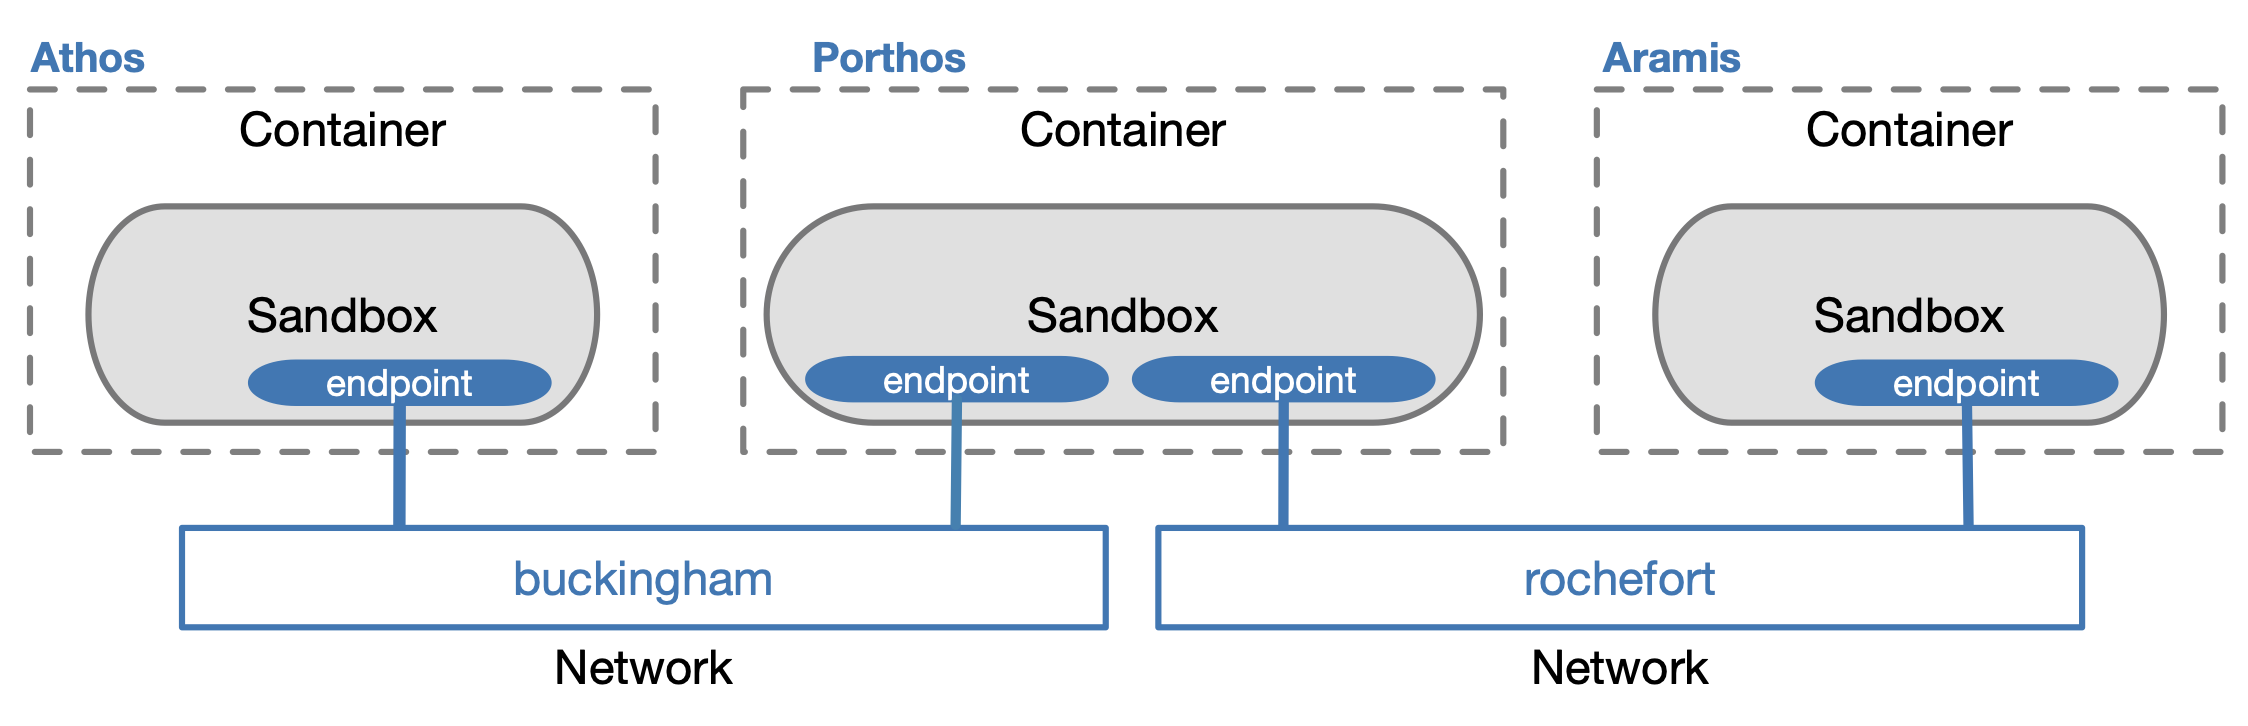
\includegraphics[width=1\linewidth]{cnm} 

}

\caption{The Docker container network model}\label{fig:cnm-docker}
\end{figure}

\begin{infobox}{exercisebox}

\textbf{Exercise}

\BeginKnitrBlock{exercise}
\phantomsection\label{exr:unnamed-chunk-29}{\label{exr:unnamed-chunk-29} }Describe the output of the following command:

\texttt{docker\ network\ ls}
\EndKnitrBlock{exercise}

\end{infobox}

Solution

\begin{infobox}{exercisebox}

The command lists all the networks created by Docker on
your computer.
For each network, the values of four attributes are shown:

\begin{itemize}
\tightlist
\item
  The identifier.
\item
  The name.
\item
  The driver used by the network.
\item
  The scope of the network (local or global).
  A local scope means that the network connects containers
  running on the same host, as opposed to a global scope that
  means that containers on different hosts can communicate.
\end{itemize}

Depending on the containers that you used
in the past, you might see different networks.
However, three networks are worth noting:

\begin{itemize}
\tightlist
\item
  The network named \textbf{bridge}, that uses the driver \textbf{bridge} and a local scope.
  By default, any new container is attached to this network.
\item
  The network named \textbf{host}, that uses the driver \textbf{host} and a local scope.
  It's used when we want a container to directly use the network interface of the host.
  It's important to remember that this network should only be used when analyzing the
  host's network traffic. In the other cases, using this network exposes
  the container to all sorts of security risks.
\item
  The network named \textbf{none}, that uses the driver \textbf{null} and a local scope.
  Attaching a container to this network means that the container
  isn't connected to any network, and therefore it's completely isolated.
\end{itemize}

\end{infobox}

\begin{infobox}{exercisebox}

\textbf{Exercise}

\BeginKnitrBlock{exercise}
\phantomsection\label{exr:unnamed-chunk-30}{\label{exr:unnamed-chunk-30} }The following command:

\texttt{docker\ network\ inspect\ bridge}

outputs the configuration of the network \textbf{bridge}.
By looking at this configuration, can you tell
what IP addresses will be given to the containers attached to this
network? What's the IP address of the router of this network?
\EndKnitrBlock{exercise}

\end{infobox}

Solution

\begin{infobox}{exercisebox}

The information is specified in the field named \textbf{IPAM}, more specifically:

\begin{itemize}
\item
  \textbf{Subnet} indicates the range of IP addresses used by the network.
  The value of this field should be 172.17.0.0/16;
  the addresses range from 172.17.0.1 to 172.17.255.255.
\item
  \textbf{Gateway} indicates the IP address of the router of the network.
  The value should be 172.17.0.1
\end{itemize}

\end{infobox}

\subsection{Creating networks}\label{creating-networks}

By default, any new container is attached to the network named \emph{bridge}.

\begin{infobox}{exercisebox}

\BeginKnitrBlock{exercise}
\phantomsection\label{exr:unnamed-chunk-31}{\label{exr:unnamed-chunk-31} }
Explain why it is not a good practice to
attach all our containers to the same network.
\EndKnitrBlock{exercise}

\end{infobox}

Solution

\begin{infobox}{exercisebox}
All new containers will be able to communicate over this network.
This is not a good idea.
If a hacker can compromise any of these containers, s/he might
be able to attack the other containers as well.
As a rule of thumb, we should attach two containers to the same network \textbf{only} on a
need-to-communicate basis.

\end{infobox}

In order to create a new network, you can use the following command:

\texttt{docker\ network\ create\ network\_name}

\begin{infobox}{exercisebox}

\textbf{Exercise}

\BeginKnitrBlock{exercise}
\phantomsection\label{exr:unnamed-chunk-32}{\label{exr:unnamed-chunk-32} }Create two networks named \emph{buckingham} and \emph{rochefort} that
use the driver \emph{bridge} (see figure \ref{fig:cnm-docker}).
By using the \texttt{docker\ network\ inspect} command,
look at the IP addresses of the new networks and write them down.
\EndKnitrBlock{exercise}

\end{infobox}

Solution

\begin{infobox}{exercisebox}
Just run the following commands:

\texttt{docker\ network\ create\ buckingham}

\texttt{docker\ network\ create\ rochefort}

The IP addresses for the network \emph{buckingham} are
172.18.0.0/16 (addresses from 172.18.0.1 to 172.18.255.255);
The IP addresses for the network \emph{rochefort} are:
172.19.0.0/16 (assuming that you create \emph{buckingham}
before \emph{rochefort}).

The IP addresses may be different on your machines.

\end{infobox}

\begin{infobox}{exercisebox}

\textbf{Exercise}

\BeginKnitrBlock{exercise}
\phantomsection\label{exr:unnamed-chunk-33}{\label{exr:unnamed-chunk-33} }Create three containers \emph{athos}, \emph{porthos} and \emph{aramis} and attach them
to the two networks \emph{buckingham} and \emph{rochefort} as displayed
in figure \ref{fig:cnm-docker}.
\textbf{The three containers will open a Linux Alpine shell}.
You'll need to launch the commands in three separate tabs of your terminal window.

\begin{itemize}
\tightlist
\item
  What will the IP addresses of the three containers be in the two networks?
  Remember that \emph{porthos} is attached to two networks, therefore it'll have two
  network interfaces (endpoints) and, as a result, two IP addresses.
\end{itemize}

\begin{itemize}
\tightlist
\item
  Verify your answers by inspecting the two networks (use the
  command \texttt{docker\ network\ inspect}).
\end{itemize}
\EndKnitrBlock{exercise}

\end{infobox}

Solution

\begin{infobox}{exercisebox}
Here are the commands to run \emph{athos} and \emph{aramis} while connecting
them to \emph{buckingham} and \emph{rochefort} respectively.

\texttt{docker\ run\ -\/-rm\ -it\ -\/-name\ athos\ -\/-network\ buckingham\ \ alpine}

\texttt{docker\ run\ -\/-rm\ -it\ -\/-name\ aramis\ -\/-network\ rochefort\ \ \ alpine}

Here's the command to run \emph{porthos} and attach it to
\emph{buckingham}:

\texttt{docker\ run\ -\/-rm\ -it\ -\/-name\ porthos\ -\/-network\ buckingham\ \ \ alpine}

The following command attaches \emph{porthos} to the second network \emph{rochefort}:

\texttt{docker\ network\ connect\ rochefort\ porthos}

As for the IP addresses, each network has IP addresses
in the range 172.x.0.0/16, where x is 18 in the
network \emph{buckingham} and 19 in the network \emph{rochefort}.
The address 172.x.0.1 is reserved for the router.
Therefore, the containers will be assigned
IP addresses from 172.x.0.2.
In this solution, we created \emph{athos}, \emph{aramis} and \emph{portos}
in this order.
Therefore, the IP addresses will be:

\begin{itemize}
\tightlist
\item
  In network \emph{buckingham}:

  \begin{itemize}
  \tightlist
  \item
    \emph{athos}: 172.18.0.2
  \item
    \emph{porthos}: 172.18.0.3
  \end{itemize}
\item
  In network \emph{rochefort}:

  \begin{itemize}
  \tightlist
  \item
    \emph{aramis}: 172.19.0.2
  \item
    \emph{porthos}: 172.19.0.3
  \end{itemize}
\end{itemize}

You can actually verify this configuration by inspecting
the two networks with the following commands:

\texttt{docker\ network\ inspect\ buckingham}

\texttt{docker\ network\ inspect\ rochefort}

The IP addresses might be different on your machines.

\end{infobox}

\subsection{Communication between containers}\label{communication-between-containers}

Let's see if and when the three containers can communicate.

\begin{infobox}{exercisebox}

\textbf{Exercise}

\BeginKnitrBlock{exercise}
\phantomsection\label{exr:unnamed-chunk-34}{\label{exr:unnamed-chunk-34} }Which containers are able to communicate?
Justify your answer.
\EndKnitrBlock{exercise}

\end{infobox}

Solution

\begin{infobox}{exercisebox}
The only containers that cannot communicate are \emph{athos} and \emph{aramis},
because they're not connected to the same network.

\end{infobox}

\begin{infobox}{exercisebox}

\textbf{Exercise}

\BeginKnitrBlock{exercise}
\phantomsection\label{exr:unnamed-chunk-35}{\label{exr:unnamed-chunk-35} }Try to ping \emph{porthos} from \emph{athos} by using its IP address.

\begin{itemize}
\tightlist
\item
  Which IP address of \emph{porthos} would you use?
\end{itemize}
\EndKnitrBlock{exercise}

\end{infobox}

Solution

\begin{infobox}{exercisebox}
We need to use the IP address assigned to the endpoint linking
\emph{porthos} to the network \emph{buckingham}, to which \emph{athos} is connected.
In our case, this is 172.18.0.3.

\end{infobox}

\begin{infobox}{exercisebox}

\textbf{Exercise}

\BeginKnitrBlock{exercise}
\phantomsection\label{exr:unnamed-chunk-36}{\label{exr:unnamed-chunk-36} }Try to ping \emph{porthos} from \emph{athos} by using its name.
Do you succeed? Are you surprised?
\EndKnitrBlock{exercise}

\end{infobox}

Solution

\begin{infobox}{exercisebox}
We succeed. Indeed, the network \emph{buckingham} provides a DNS server, that
can translate names into IP addresses.

\end{infobox}

You can now exit the three containers.

\end{document}
